\chapter{AVL Trees}
\label{ch:avl}

\newcommand{\lecnum}{16}
%\newcommand{\lectitle}{AVL Trees}
\newcommand{\lecturer}{Frank Pfenning}

\chapterTAGS{avl, complexity, correctness, dictionary, ds-invariant, safety, search, testing}
\maketitle

\begin{preamble}
\noindent
Binary search trees are an excellent data structure to implement
associative arrays, maps, sets, and similar interfaces.  The main
difficulty is that they are efficient only when they are balanced.
Straightforward sequences of insertions can lead to highly unbalanced
trees with poor asymptotic complexity and unacceptable practical
efficiency.  For example, if we insert $n$ entries with keys that are
in strictly increasing or decreasing order, the complexity for $n$
insertions will be $O(n^2)$.  On the other hand, if we can keep the
height to $O(\log n)$, as it is for a perfectly balanced tree, then
the complexity is bounded by $O(n\log n)$.

The tree can be kept balanced by dynamically \emph{rebalancing} the
search tree during insert or search operations.  We have to be careful
not to destroy the ordering invariant of the tree while we rebalance.
Because of the importance of binary search trees, researchers have
developed many different algorithms for keeping trees in balance, such
as AVL trees, red/black trees, splay trees, or randomized binary
search trees.  They differ in the invariants they maintain (in
addition to the ordering invariant), and when and how the rebalancing
is done.

In this lecture we use \emph{AVL trees}, which is a simple and
efficient data structure to maintain balance, and is also the first
that has been proposed.  It is named after its inventors,
G.M. Adelson-Velskii and E.M. Landis, who described it in 1962.
\end{preamble}

\begin{gram}[Learning Goals]
In terms of the learning objectives of the course, AVL trees make the
following contributions:
\begin{description}
\item[Computational Thinking: ]%
  We learn that the computational limitations of a data structure (here the
  possibility that binary search trees can develop a linear behavior) can
  sometime be overcome through clever thinking (here rebalancing).

\item[Algorithms and Data Structures: ]%
  We examine AVL trees as an example of self-balancing trees.

\item[Programming: ]%
  We use contracts to guide the implementation of code with increasingly
  complex invariants.
\end{description}
\end{gram}


\section{The Height Invariant}
\label{sec:avl:height_invariant}
\TAGS{avl, ds-invariant}

Recall the \emph{ordering invariant} for binary search trees.
\begin{quote}
  \noindent\textbf{Ordering Invariant.} At any node with key $k$ in a
  binary search tree, all keys of the entries in the left subtree are
  strictly less than $k$, while all keys of the entries in the right
  subtree are strictly greater than $k$.
\end{quote}

To describe AVL trees we need the concept of \emph{tree height}, which
we define as the maximal length of a path from the root to a leaf.  So
the empty tree has height $0$, the tree with one node has height $1$,
a balanced tree with three nodes has height $2$.  If we add one more
node to this last tree is will have height $3$.  Alternatively, we can
define it recursively by saying that the empty tree has height $0$,
and the height of any node is one greater than the maximal height of
its two children.  AVL trees maintain a \emph{height invariant} (also
sometimes called a \emph{balance invariant}).
\begin{quote}
  \noindent\textbf{Height Invariant.} At any node in the tree,
  the heights of the left and right subtrees differ by at most 1.
\end{quote}

As an example, consider the following binary search tree of height 3.
\begin{center}
  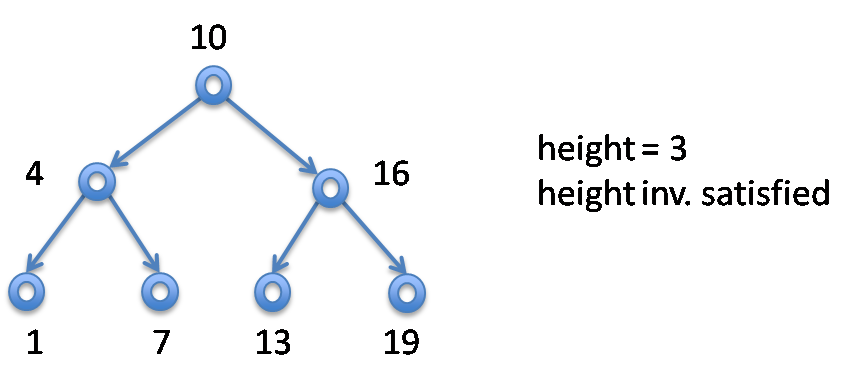
\includegraphics[width=0.75\textwidth]{img/avl1.png}
\end{center}
If we insert a new entry with a key of $14$, the insertion algorithm
for binary search trees without rebalancing will put it to the
right of $13$.
\begin{center}
  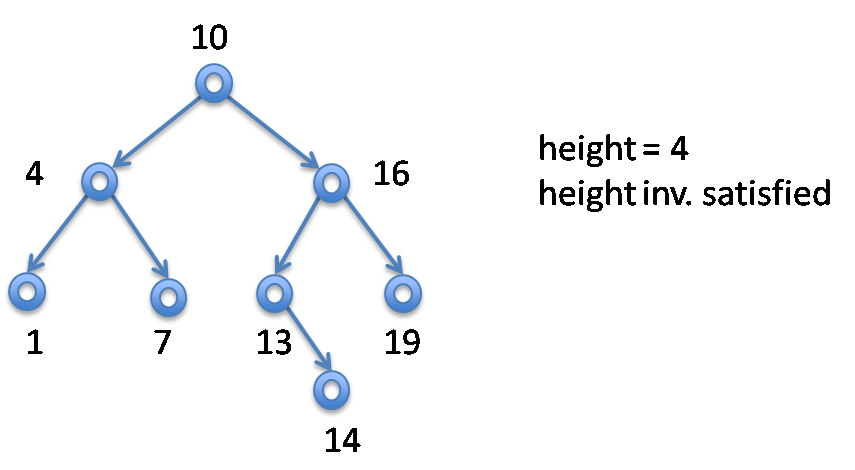
\includegraphics[width=0.75\textwidth]{img/avl2.png}
\end{center}
Now the tree has height 4, and one path is longer than the others.
However, it is easy to check that at each node, the height of the
left and right subtrees still differs only by one.  For example,
at the node with key $16$, the left subtree has height 2 and the right
subtree has height 1, which still obeys our height invariant.

Now consider another insertion, this time of an entry with key $15$.
This is inserted to the right of the node with key 14.
\begin{center}
  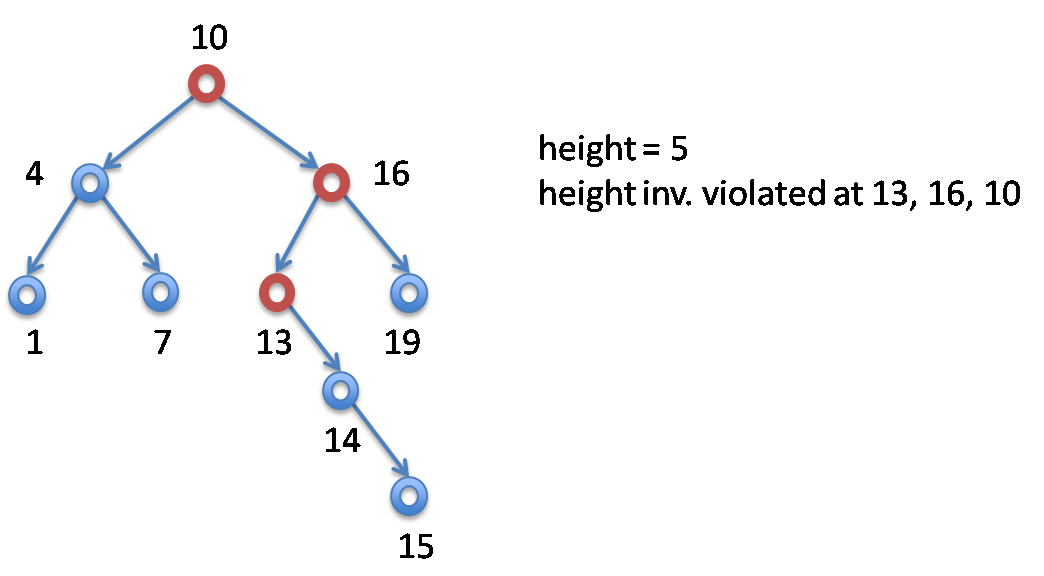
\includegraphics[width=0.75\textwidth]{img/avl3.png}
\end{center}
All is well at the node labeled 14: the left subtree has height 0
while the right subtree has height 1.  However, at the node labeled
13, the left subtree has height 0, while the right subtree has height
2, violating our invariant.  Moreover, at the node with key 16, the
left subtree has height 3 while the right subtree has height 1, also a
difference of 2 and therefore an invariant violation.

We therefore have to take steps to rebalance the tree.  We can see without
too much trouble that we can restore the height invariant if we move
the node labeled 14 up and push node 13 down and to the left,
resulting in the following tree.
\begin{center}
  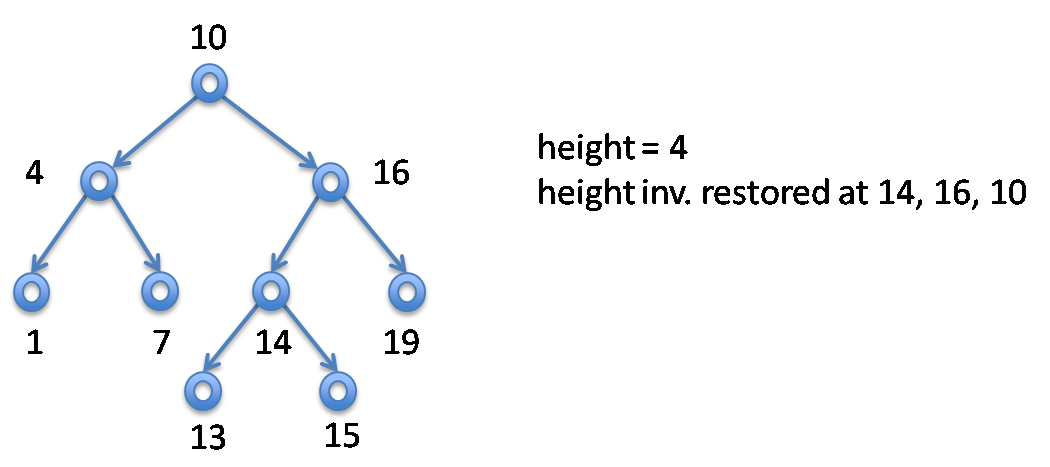
\includegraphics[width=0.9\textwidth]{img/avl4.png}
\end{center}

The question is how to do this in general.  In order to understand
this we need a fundamental operation called a \emph{rotation}, which
comes in two forms, \emph{left rotation} and \emph{right rotation}.

\section{Left and Right Rotations}
\label{sec:avl:rotations}
\TAGS{avl, ds-invariant}

Below, we show the situation before a left rotation.  We have
generically denoted the crucial key values in question with $x$ and
$y$.  Also, we have summarized whole subtrees with the intervals
bounding their key values.  At the root of the subtree we can have
intervals that are unbounded on the left or right.  We denote these
with pseudo-bounds $-\infty$ on the left and $+\infty$ on the right.
We then write $\alpha$ for a left endpoint which could either be an
integer or $-\infty$ and $\omega$ for a right endpoint which could be
either an integer of $+\infty$.  The tree on the right is after the
left rotation.
\begin{center}
  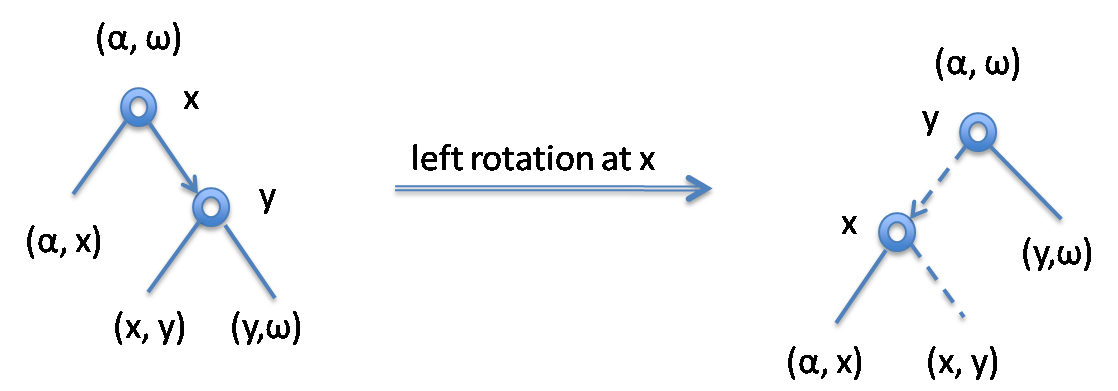
\includegraphics[width=0.99\textwidth]{img/avl5.png}
\end{center}
From the intervals we can see that the ordering invariants are
preserved, as are the contents of the tree.  We can also see that it
shifts some nodes from the right subtree to the left subtree.  We
would invoke this operation if the invariants told us that we have
to rebalance from right to left.

We implement this with some straightforward code.  First, recall
the type of trees from last lecture.  We do not repeat the functions
\lstinline'is_tree' that checks the basic structure of a tree and
\lstinline'is_ordered' that checks if a tree is ordered.
\begin{lstlisting}[language={[C0]C}]
struct tree_node {
  entry data;
  struct tree_node* left;
  struct tree_node* right;
};
typedef struct tree_node tree;
bool is_tree(tree* T);
bool is_ordered(tree* T, entry lo, entry hi);
\end{lstlisting}
The main point to
keep in mind is to use (or save) a component of the input before
writing to it.  We apply this idea systematically, writing to
a location immediately after using it on the previous line.
\begin{lstlisting}[language={[C0]C}]
tree* rotate_left(tree* T)
//@requires T != NULL && T->right != NULL;
{
  tree* R = T->right;
  T->right = T->right->left;
  R->left = T;
  return R;
}
\end{lstlisting}
%\begin{lstlisting}
%tree* rotate_left(tree* T)
%//@requires is_ordtree(T);
%//@requires T != NULL && T->right != NULL;
%//@ensures is_ordtree(\result);
%//@ensures \result != NULL && \result->left != NULL;
%{
%  tree* root = T->right;
%  T->right = root->left;
%  root->left = T;
%  fix_height(root->left);	/* must be first */
%  fix_height(root);
%  return root;
%}
%\end{lstlisting}
These rotations work generically.  When we apply them to AVL trees
specifically later in this lecture, we will also have to recalculate
the heights of the two nodes involved.  This involves only looking up
the height of their children.

The right rotation is exactly the inverse.  First in pictures:
\begin{center}
  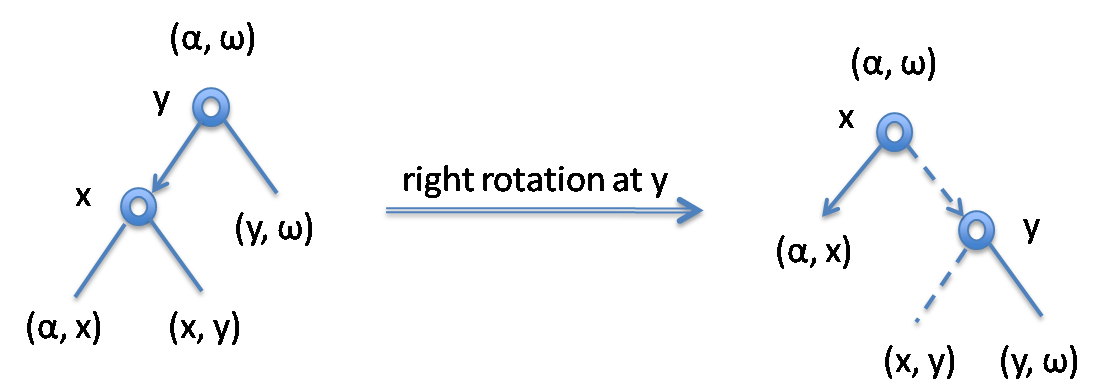
\includegraphics[width=0.99\textwidth]{img/avl6.png}
\end{center}
Then in code:
\begin{lstlisting}[language={[C0]C}]
tree* rotate_right(tree* T)
//@requires T != NULL && T->left != NULL;
{
  tree* R = T->left;
  T->left = T->left->right;
  R->right = T;
  return R;
}
\end{lstlisting}
%\begin{lstlisting}[numbers=left]
%tree* rotate_right(tree* T)
%//@requires is_ordtree(T);
%//@requires T != NULL && T->left != NULL;
%//@ensures is_ordtree(\result);
%//@ensures \result != NULL && \result->right != NULL;
%{
%  tree* root = T->left;
%  T->left = root->right;
%  root->right = T;
%  fix_height(root->right);	/* must be first */
%  fix_height(root);
%  return root;
%}
%\end{lstlisting}


\section{Searching for a Key}
\label{sec:avl:searching}
\TAGS{avl, dictionary, search}

Searching for a key in an AVL tree is identical to searching for it in a plain
binary search tree.  We only need the ordering invariant to find the entry;
the height invariant is only relevant for inserting an entry.


\section{Inserting an Entry}
\label{sec:avl:inserting}
\TAGS{avl, ds-invariant}

The basic recursive structure of inserting an entry is the same as
for searching for an entry.  We compare the entry's key with the
keys associated with the nodes of the trees, inserting recursively
into the left or right subtree.  When we find an entry with the
exact key we overwrite the entry in that node.  If we encounter a
null tree, we construct a new tree with the entry to be inserted and
no children and then return it.  As we return the new subtrees (with
the inserted entry) towards the root, we check if we violate the
height invariant.  If so, we rebalance to restore the invariant and
then continue up the tree to the root.

The main cleverness of the algorithm lies in analyzing the situations
when we have to rebalance and need to apply the appropriate rotations to
restore the height invariant.  It turns out that one or two rotations
on the whole tree always suffice for each insert operation, which is
a very elegant result.

First, we keep in mind that the left and right subtrees' heights
before the insertion can differ by at most one.  Once we insert an
entry into one of the subtrees, they can differ by at most two.  We
now draw the trees in such a way that the height of a node is
indicated by the height that we are drawing it at.

The first situation we describe is where we insert into the right
subtree, which is already of height $h+1$ where the left subtree has
height $h$.  If we are unlucky, the result of inserting into the right
subtree will give us a new right subtree of height $h+2$ which raises
the height of the overall tree to $h+3$, violating the height
invariant.  This situation is depicted below.  Note that the node we
inserted does not need to be $z$, but there must be a node $z$ in
the indicated position.
\begin{center}
  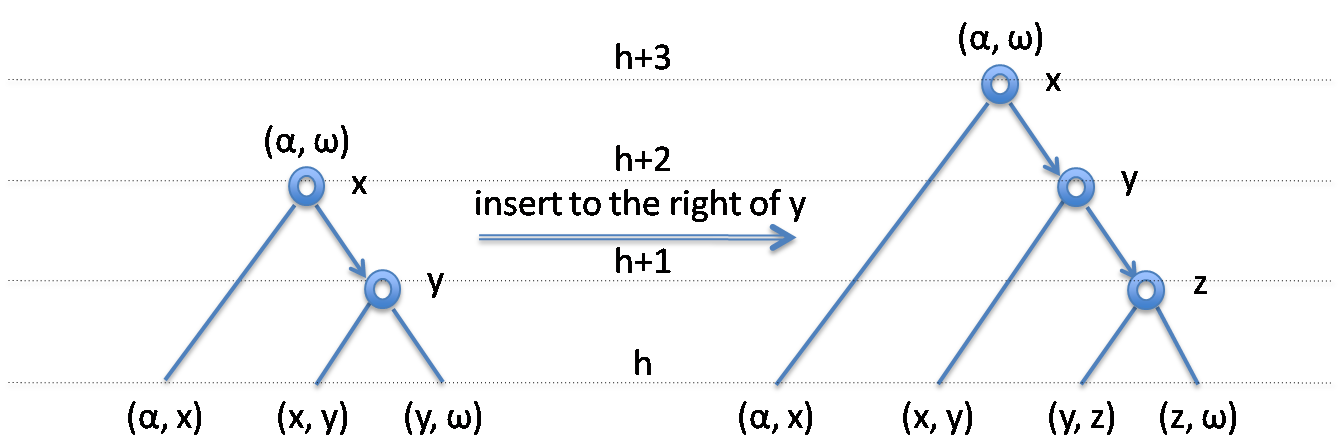
\includegraphics[width=0.99\textwidth]{img/avl7a.png}
\end{center}
If the new right subtree has height $h+2$, either its right or its
left subtree must be of height $h+1$ (and only one of them --- think
about why). If it is the right subtree we are in the situation
depicted on the right above (and on the left below).  While the trees
$(\alpha, x)$ and $(x, y)$ must have exactly height $h$, the trees
$(y, z)$ and $(z, \omega)$ need not.  However, they differ by at most
1, because we are investigating the case where the lowest place in
the tree where the invariant is violated is at $x$.
\begin{center}
  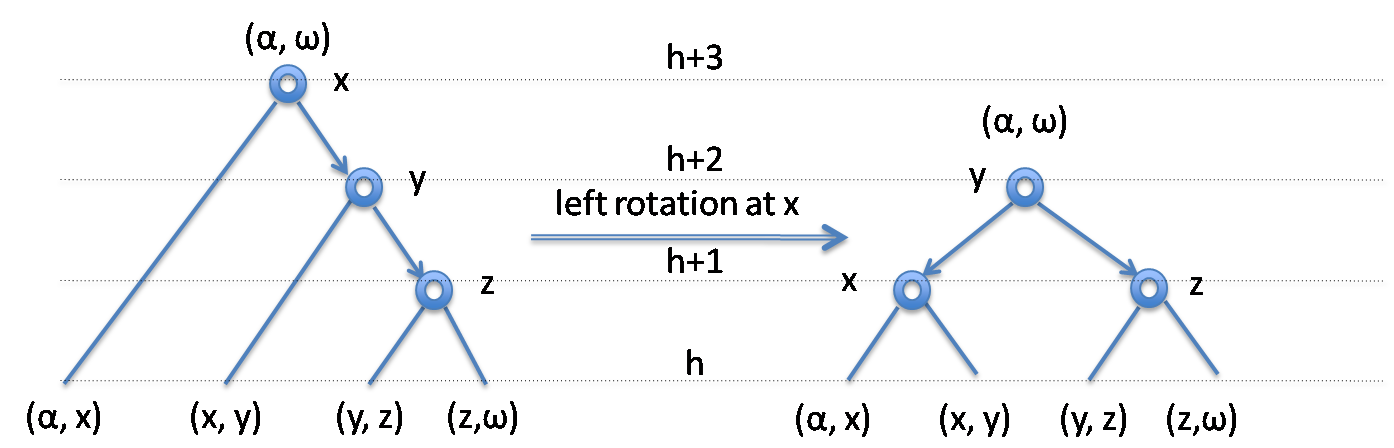
\includegraphics[width=0.99\textwidth]{img/avl7.png}
\end{center}
We fix this with a left rotation at $x$, the result of which is displayed to
the right.  Because the height of the overall tree is reduced to its
original $h+2$, no further rotation higher up in the tree will be
necessary.

In the second case we consider, we insert to the \emph{left} of the
right subtree, and the result has height $h+1$.  This situation is
depicted on the right below.
\begin{center}
  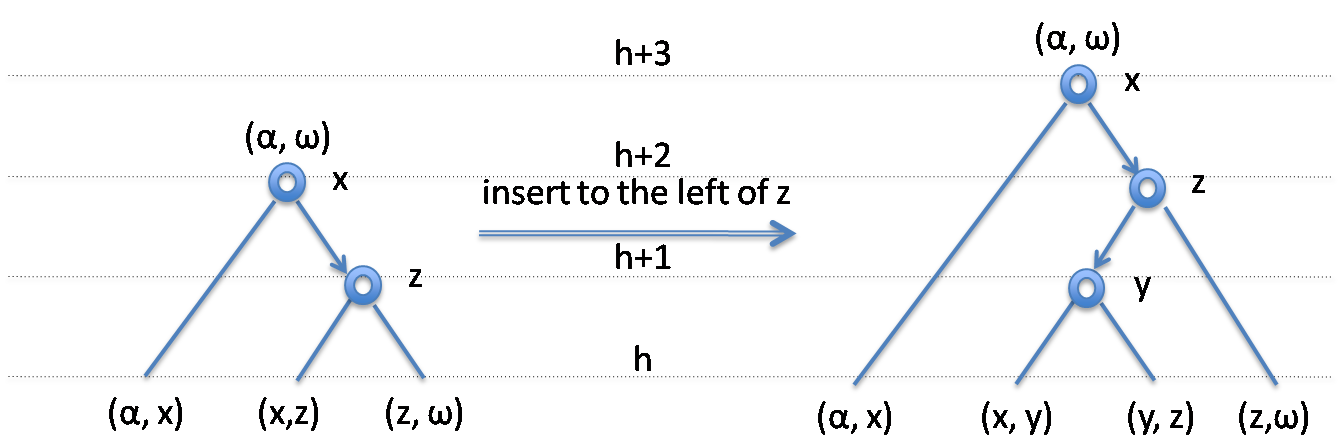
\includegraphics[width=0.99\textwidth]{img/avl8b.png}
\end{center}
In the situation on the right, the subtrees labeled $(\alpha, x)$ and
$(z, \omega)$ must have exactly height $h$, but only one of $(x,y)$
and $(y,z)$ does.  In this case, a single left rotation alone will not
restore the invariant (see Exercise~\ref{exc:left-not-restore}).
Instead, we apply a so-called \emph{double rotation}: first a
\emph{right} rotation at $z$, then a \emph{left} rotation at the root
labeled $x$.  When we do this we obtain the picture on the right,
restoring the height invariant.
\begin{center}
  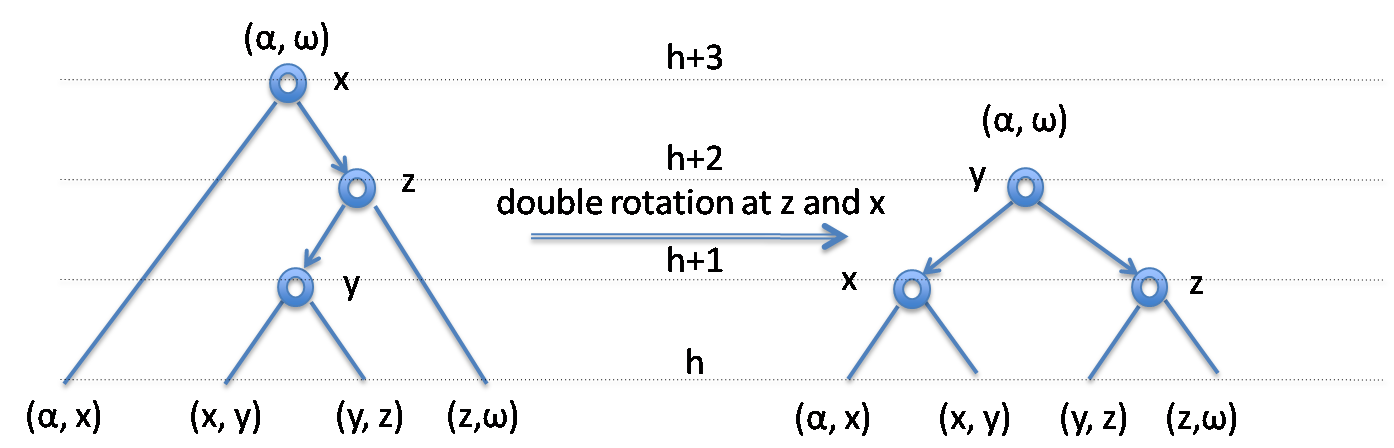
\includegraphics[width=0.99\textwidth]{img/avl8.png}
  \label{dia:RL}
\end{center}
There are two additional symmetric cases to consider, if we insert
the new entry on the left (see Exercise~\ref{exc:insert-left}).

We can see that in each of the possible cases where we have to restore
the invariant, the resulting tree has the same height $h+2$ as before
the insertion.  Therefore, the height invariant \emph{above} the place
where we just restored it will be automatically satisfied, without any
further rotations.


\section{Checking Invariants}
\label{sec:avl:checkinvariant}
\TAGS{avl, correctness, ds-invariant, safety}

The interface for the implementation is \emph{exactly} the same as for
binary search trees, as is the code for searching for a key.
In various places in the algorithm we have to compute the
height of the tree.  This could be an operation of asymptotic
complexity $O(n)$, unless we store it in each node and just
look it up.  So we have:

\begin{lstlisting}[language={[C0]C}]
typedef struct tree_node tree;
struct tree_node {
  entry data;
  int height;          // New
  tree* left;
  tree* right;
};

/* height(T) returns the precomputed height of T in O(1) */
int height(tree* T) {
  return T == NULL ? 0 : T->height;
}
\end{lstlisting}
The conditional expression %
$b$ \lstinline'?' $e_1 $\lstinline' : '$e_2$ %
evaluates to the result of $e_1$ if the boolean test $b$
returns \lstinline'true' and to the value of $e_2$ if it returns
\lstinline'false'.

When checking if a tree is balanced, we check that all the heights
that have been computed are correct.
\begin{lstlisting}[language={[C0]C}]
bool is_specified_height(tree* T) {
  if (T == NULL) return true;
  return is_specified_height(T->left)
      && is_specified_height(T->right)
      && T->height == max(height(T->left),
                         height(T->right)) + 1;
}

bool is_balanced(tree* T) {
  if (T == NULL) return true;
  return abs(height(T->left) - height(T->right)) <= 1
      && is_balanced(T->left) && is_balanced(T->right);
}
\end{lstlisting}

A tree is an AVL tree if it is both ordered (as defined and
implemented in the BST lecture, and extended by our
\lstinline'is_specified_height' condition) and balanced.
\begin{lstlisting}[language={[C0]C}]
bool is_avl(tree* T) {
  return is_tree(T) && is_ordered(T, NULL, NULL)
      && is_specified_height(T)
      && is_balanced(T);
}
\end{lstlisting}

Of course, if we store the height of the trees for fast access, we need to
adapt it when rotating trees.  After all, the whole purpose of tree rotations
is to rebalance and change the height.  For that, we implement a function
\lstinline'fix_height' that computes the height of a tree from the height of
its children.  Its implementation directly follows the definition of the
height of a tree.
\begin{lstlisting}[language={[C0]C}]
void fix_height(tree* T)
//@requires T != NULL;
//@requires is_specified_height(T->left);
//@requires is_specified_height(T->right);
{
  int hl = height(T->left);
  int hr = height(T->right);
  T->height = (hl > hr ? hl+1 : hr+1);
  return;
}
\end{lstlisting}

The implementation of \lstinline'rotate_right' and
\lstinline'rotate_left' needs to be adapted to include calls to
\lstinline'fix_height'. These calls need to compute the heights of the
children first, before computing that of the root, because the height of the
root depends on the height we had previously computed for the child. Hence, we
need to update the height of the child before updating the height of the root.
For example, \lstinline'rotate_left' is upgrades as follows
\newpage
\begin{lstlisting}[language={[C0]C}]
tree* rotate_left(tree* T)
//@requires T != NULL && T->right != NULL;
//@requires is_specified_height(T->left);
//@requires is_specified_height(T->right);
//@ensures is_specified_height(\result);
{
  tree* R = T->right;
  T->right = T->right->left;
  R->left = T;
  fix_height(T);
  fix_height(R);
  return R;
}
\end{lstlisting}


We use this, for example, in a utility function that creates
a new leaf from an entry (which may not be \lstinline'NULL').
%\begin{lstlisting}[language={[C0]C}]
%tree* leaf(entry e)
%//@requires e != NULL;
%//@ensures is_avl(\result);
%{ tree* T = alloc(struct tree_node);
%  T->data = e;
%  T->height = 1;
%  T->left = NULL;
%  T->right = NULL;
%  return T;
%}
%\end{lstlisting}
\begin{lstlisting}[language={[C0]C}]
tree* leaf(entry e)
//@requires e != NULL;
//@ensures is_avl(\result);
{
  tree* T = alloc(tree);
  T->data = e;
  T->height = 1;
  return T;
}
\end{lstlisting}
Recall that the pointer fields are set to \lstinline'NULL' by default when the
structure is allocated.


\newpage
\section{Implementing Insertion}
\label{sec:avl:insertion_impl}
\TAGS{avl, correctness, ds-invariant, safety}

The code for inserting an entry into the tree is mostly identical
to the code for plain binary search trees.  The difference is that
after we insert into the left or right subtree, we call a function
\lstinline'rebalance_left' or \lstinline'rebalance_right', respectively, to
restore the invariant if necessary and calculate the new height.
\begin{lstlisting}[language={[C0]C}]
tree* tree_insert(tree* T, entry e)
//@requires is_avl(T) && e != NULL;
//@ensures is_avl(\result);
{
  if (T == NULL) return leaf(e);

  //@assert is_avl(T->left);
  //@assert is_avl(T->right);
  int cmp = key_compare(entry_key(e), entry_key(T->data));
  if (cmp == 0) {        // Found
    T->data = e;
  } else if (cmp < 0) {  // Go left
    T->left = tree_insert(T->left, e);
    //@assert is_avl(T->left);
    T = rebalance_left(T);                // New
    //@assert is_avl(T);
  } else if (cmp > 0) {  // Go right
    T->right = tree_insert(T->right, e);
    //@assert is_avl(T->right);
    T = rebalance_right(T);               // New
    //@assert is_avl(T);
  }
  return T;
}
\end{lstlisting}
%\begin{lstlisting}[language={[C0]C}]
%tree* tree_insert(tree* T, entry e)
%//@requires is_avl(T);
%//@requires e != NULL;
%//@ensures is_avl(\result);
%{
%  if (T == NULL) {
%    T = leaf(e);		/* create new leaf with data e */
%  } else {
%    int r = key_compare(entry_key(e), entry_key(T->data));
%    if (r < 0) {
%      T->left = tree_insert(T->left, e);
%      T = rebalance_left(T);	/* also fixes height */
%    } else if (r == 0) {
%      T->data = e;
%    } else { //@assert r > 0;
%      T->right = tree_insert(T->right, e);
%      T = rebalance_right(T);	/* also fixes height */
%    }
%  }
%  return T;
%}
%\end{lstlisting}
The pre- and post-conditions of this function are actually not strong
enough to prove this function correct.  We also need an assertion
about how the tree might change due to insertion, which is somewhat
tedious.  If we perform dynamic checking with the contract above,
however, we establish that the result is indeed an AVL tree.  As we
have observed several times already: we can test for the desired
property, but we may need to strengthen the pre- and post-conditions
in order to rigorously prove it.

\newpage
We show only the function \lstinline'rebalance_right';
\lstinline'rebalance_left' is symmetric.
\begin{lstlisting}[language={[C0]C}]
tree* rebalance_right(tree* T)
//@requires T != NULL && T->right != NULL;
//@requires is_avl(T->left) && is_avl(T->right);
//@ensures is_avl(\result);
{
  if (height(T->right) - height(T->left) == 2) {
    if (height(T->right->right) > height(T->right->left)) {
      // Single rotation
      T = rotate_left(T);
    } else {
      //@assert height(T->right->left) > height(T->right->right);
      // Double rotation
      T->right = rotate_right(T->right);
      T = rotate_left(T);
    }
  } else { // No rotation needed, but tree may have grown
    fix_height(T);
  }
  return T;
}
\end{lstlisting}
%\begin{lstlisting}[language={[C0]C}]
%tree* rebalance_right(tree* T)
%//@requires T != NULL;
%//@requires is_avl(T->left) && is_avl(T->right);
%/* also requires that T->right is result of insert into T */
%//@ensures is_avl(\result);
%{
%  tree* l = T->left;
%  tree* r = T->right;
%  int hl = height(l);
%  int hr = height(r);
%  if (hr > hl+1) {
%    //@assert hr == hl+2;
%    if (height(r->right) > height(r->left)) {
%      //@assert height(r->right) == hl+1;
%      T = rotate_left(T);
%      //@assert height(T) == hl+2;
%      return T;
%    } else {
%      //@assert height(r->left) == hl+1;
%      /* double rotate left */
%      T->right = rotate_right(T->right);
%      T = rotate_left(T);
%      //@assert height(T) == hl+2;
%      return T;
%    }
%  } else { //@assert !(hr > hl+1);
%    fix_height(T);
%    return T;
%  }
%}
%\end{lstlisting}

Note that the preconditions are weaker than we would like.  In
particular, they do not imply some of the assertions we have added in
order to show the correspondence to the pictures.  This is left as the
(difficult) Exercise~\ref{exc:avl-invs}.  Such assertions are nevertheless
useful because they document expectations based on informal reasoning
we do behind the scenes.  Then, if they fail, they may be evidence
for some error in our understanding, or in the code itself, which
might otherwise go undetected.


\section{Experimental Evaluation}
\label{sec:avl:exp_eval}
\TAGS{avl, complexity, testing}

We would like to assess the asymptotic complexity and then
experimentally validate it.  It is easy to see that both insert and
lookup operations take time $O(h)$, where $h$ is the height of the
tree.  But how is the height of the tree related to the number of
entries stored, if we use the balance invariant of AVL trees?  It
turns out that $h$ is $O(\log{n})$.  It is not difficult to
prove this, but it is beyond the scope of this course.

To experimentally validate this prediction, we have to run the code
with inputs of increasing size.  A convenient way of doing this is to
double the size of the input and compare running times.  If we insert
$n$ entries into the tree and look them up, the running time should
be bounded by $c \times n \times \log{n}$ for some constant $c$.
Assume we run it at some size $n$ and observe $r = c \times n \times
\log{n}$.  If we double the input size we have $c \times (2 \times n)
\times \log{(2 \times n)} = 2 \times c \times n \times (1+\log{n}) = 2
\times r + 2 \times c \times n$, we mainly expect the running time to
double with an additional summand that roughly doubles as $n$ doubles.
In order to smooth out minor variations and get bigger numbers, we run
each experiment 100 times.  Here is the table with the results:
\[\renewcommand{\arraystretch}{1.25}
\begin{array}{|l|r|l|r|}\hline
n & \mbox{AVL trees} & \mbox{increase} & \mbox{BSTs} \\ \hline\hline
2^9 & 0.129 & {-} & 1.018 \\ \hline
2^{10} & 0.281 & 2r+0.023 & 2.258 \\ \hline
2^{11} & 0.620 & 2r+0.058 & 3.094 \\ \hline
2^{12} & 1.373 & 2r+0.133 & 7.745 \\ \hline
2^{13} & 2.980 & 2r+0.234 & 20.443 \\ \hline
2^{14} & 6.445 & 2r+0.485 & 27.689 \\ \hline
2^{15} & 13.785 & 2r+0.895 & 48.242\\ \hline
\end{array}\]
We see in the third column, where $2r$ stands for the doubling of the
previous value, we are quite close to the predicted running time,
with a approximately linearly increasing additional summand.

In the fourth column we have run the experiment with plain binary
search trees which do not rebalance automatically.  First of all, we
see that they are much less efficient, and second we see that their
behavior with increasing size is difficult to predict, sometimes
jumping considerably and sometimes not much at all.  In order to
understand this behavior, we need to know more about the order and
distribution of keys that were used in this experiment.  They were
strings, compared lexicographically.  The keys were generated by
counting integers upward and then converting them to strings.  The
distribution of these keys is haphazard, but not random.  For example,
if we start counting at $0$
\begin{lstlisting}[language={[C0]C}]
"0" < "1" < "2" < "3" < "4" < "5" < "6" < "7" < "8" < "9"
     < "10" < "12" < ...
\end{lstlisting}
the first ten strings are in ascending order but then numbers
are inserted between \lstinline'"1"' and \lstinline'"2"'.  This kind of
haphazard distribution is typical of many realistic applications,
and we see that binary search trees without rebalancing perform
quite poorly and unpredictably compared with AVL trees.

\bigskip

The complete code for this lecture can be found on the course website.

%\clearpage
\section{Exercises}
\label{sec:avl:exercises}

\begin{exercise}
\label{exc:left-not-restore}
Show that in the situation on page~\pageref{dia:RL} a single
left rotation at the root will not necessarily restore the
height invariant.
\end{exercise}

\begin{exercise}
\label{exc:double-rotation}
Show, in pictures, that a double rotation is a composition
of two rotations.  Discuss the situation with respect to the
height invariants after the first rotation.
\end{exercise}

\begin{exercise}
\label{exc:left-right}
Show that left and right rotations are inverses of each
other.  What can you say about double rotations?
\end{exercise}

\begin{exercise}
\label{exc:insert-left}
Show the two cases that arise when inserting into the
left subtree might violate the height invariant, and show
how they are repaired by a right rotation, or a double
rotation.  Which two single rotations does the double
rotation consist of in this case?
\end{exercise}

\begin{exercise}
\label{exc:avl-invs}
Strengthen the invariants in the AVL tree implementation
so that the assertions and postconditions which guarantee that rebalancing
restores the height invariant and reduces the height
of the tree follow from the preconditions.
\end{exercise}
